\chapter{Detecting Phishing URLs using Transformers}
\label{chp:urltran}
%\todo{Add some general information connecting to the broader theme. + Make the introduction more relevant to the thesis.}
%\todo{TODO: Make references local? For figures etc.}

In this chapter, we present our work on phishing URL (Uniform Resource Locator) detection~\citep{maneriker2021urltran} conducted at Microsoft, contextualized within the broader theme of our thesis surrounding the use of structures to build \textit{adversarial testing} for \textit{pre-deployment} robustness. 
We study the problem of detecting phishing URLs using transformer models.

Browsers often include security features to detect phishing web pages. 
In the past, some browsers evaluated unknown URLs for inclusion in lists of known phishing pages.
However, phishing URLs and websites have a very short life span~\citep{garera2007framework,chu2013protect}. 
Therefore, models must be able to \textit{adapt} to rapidly changing data distribution.
As the number of URLs and known phishing pages has continued to increase rapidly, browsers have started to include one or more machine learning classifiers in their security services, which aim to better protect end users from harm.

Recent research has proposed using deep learning models for the phishing URL detection task~\cite{sahoo2017malicious,yerima2020high,ren2019bidirectional,peng2019joint,huang2019phishing,tajaddodianfar2020texception}.
Concurrently, text embedding research using transformers has led to state-of-the-art results in many natural language processing tasks.
In this contribution, we first comprehensively analyze transformer models on the phishing URL detection task.
We consider both pre-trained and end-to-end transformer models, with standard masked language models and additional domain-specific pre-training tasks.
We compare end-to-end training compare against fine-tuned BERT and RoBERTa models.
Misclassifying a benign URL as malicious can be damaging for a phishing URL classification model.%~\cite{TODO}\todo{Fix reference}.
Therefore, phishing URL detection models are compared by measuring true positive rates at very low false positive rates.
 The insights our experiments help us propose \URLTranSys, which uses transformers to significantly improve the performance of phishing URL detection over a wide range of very low false positive rates (FPRs) compared to other deep learning-based methods.
For example, \URLTranSys yields a true positive rate (TPR) of 86.80\% compared to 71.20\% for the next best baseline at an FPR of 0.01\%, resulting in a relative improvement of over 21.9\%.
We use insights from the structure of URL grammar~\cite{rfc3986}.

As mentioned previously, phishing URL attacks are carried out through short-lived and changing URL patterns.
Therefore, the machine learning models must be retrained and redeployed at regular intervals.
This procedure may lead to a \textit{catastrophic forgetting}~\citep{mccloskey1989catastrophic} phenomenon, whereby models forget the old patterns and only adapt to new ones.
In our second contribution to this work, we propose a threat model and construct an \textit{adversarial testing} scenario to validate models against known threat patterns before deployment.
We consider some classical adversarial black-box phishing attacks, such as those based on homoglyphs and compound word splits, to improve the robustness of \URLTranSys.
Inspired by the behavioral testing paradigm~\citep{ribeiro2020beyond}, we provide algorithms to efficiently construct datasets that can help quantify the capabilities of trained models against known threat patterns.
%We consider additional fine tuning with these adversarial samples and demonstrate that \URLTranSys can maintain low FPRs under these scenarios.

\section{Introduction}
\label{sec:urltran:intro}
\todo{Background on adversarial testing at some point?} Phishing occurs when a malicious web page is created to mimic the legitimate login page used to access a popular online service for the purpose of harvesting the user's credentials or a web page whose purpose is to input credit card or other payment information.
Typical phishing targets include online banking services, web-based email portals, and social media websites.
Attackers use several methods to direct the victim to the phishing site in order to launch the attack.
In some cases, they may send the user a phishing email containing the URL of a phishing page.
Attackers may also use search engine optimization techniques to rank phishing pages high in a search result query.
Modern email platforms use various machine learning models to detect phishing web page attacks.
In this work, we propose a new deep learning model that analyzes URLs and is based on transformers which have shown state-of-the-art performance in many important natural language processing tasks.


In order to prevent users from inadvertently uploading personal information to the attackers, web browsers provide additional security services to identify and block or warn a user from visiting a known phishing page.
For example, Google's Chrome browser utilizes their Safe Browsing technology~\citep{safebrowsing_google} and Microsoft's Edge browser includes Windows Defender SmartScreen~\citep{smartscreen_microsoft}.
In a related attack which is also addressed by these services, malicious URLs may point to a web page hosted by a misconfigured or unpatched server with the goal of exploiting browser vulnerabilities in order to infect the user's computer with malware (i.e., malicious software).
Successful phishing web page detection includes a number of significant challenges.
First, there is a huge class imbalance associated with this problem.
The number of phishing pages on the internet is very small compared to the total number of web pages available to users. Second, phishing campaigns are often short-lived. In order to avoid detection, attackers may move the login page from one site to another multiple times per day.
Third, phishing attacks continue to be a persistent problem.
The number of known phishing sites continues to increase over time. Therefore, blocking phishing attacks only using a continuously growing list of known phishing sites often fails to protect users in practice.



Popular web browsers may render hundreds of millions or even billions of web pages each day.
In order to be effective, any phishing or malicious web page detection must be fast.
For this reason, several researchers~\citep{blum2020lexical,le2018malicious,tajaddodianfar2020texception} have proposed detecting both phishing and malicious web pages based solely on analyzing the URL itself.
\begin{comment}
	Phishing cyberattacks have been occurring for approximately 25 years, and their main goal remains the same today: convincing the user to disclose their credentials and financial information which the attacker can then use for their own financial gain. Phishing attacks can be initiated through emails and social media, and they target financial, online payments, social media, entertainment and technological companies. The attacker usually impersonates a known and reputable brand (e.g. Bank of America, Google, Amazon, Facebook, Microsoft) and attempts to convince the victim to disclose personal information.
\end{comment}
With the proliferation and ease of access to phishing kits sold on the black market as well as the phishing as a service offering, it has become easy for attackers with little expertise to deploy phishing sites and initiate such attacks. Consequently, phishing is currently on the rise and costing over \$57 million from more than 114,000 victims in the US according to a recent FBI report~\citeyearpar{fbi2019internet}.
The number of phishing attacks rose in Q3 of 2019 to a high level not seen since late 2016~\citep{helpnetsecurity2019phishing}.
As phishing is proving to be more and more fruitful, the attacks have become increasingly sophisticated. At the same time, the lifespan of phishing URLs has continued to drop dramatically – from 10+ hours to minutes~\citep{zvelophish2020phishing}. 


Given the significant repercussions of visiting a phishing or malicious web page, the detection of these URLs has been an active area of research~\citep{sahoo2017malicious}.
Researchers have proposed the use of extracted feature-based natural language processing methods to detect malicious URLs~\citep{blum2020lexical}.
Recent efforts have also begun to use deep learning models to detect these URLs~\citep{le2018malicious,tajaddodianfar2020texception}.
%URLNet~\citep{le2018malicious} is a deep convolutional neural network (CNN) and includes separate character and word-level models for the malicious URL detection task.
%The Texception~\citep{tajaddodianfar2020texception} model, which is used to detect phishing URLs,extends some ideas in URLNet by including small kernels which can be deployed in a wide variety of configurations in terms of width, depth or both.
Concurrently, semi-supervised machine learning methods have been used to create text embeddings that offer state-of-the-art results in many natural language processing tasks.
The key idea in these approaches is the inclusion of a transformer model~\citep{vaswani2017attention}.
BERT~\citep{devlin2019bert,rogers2020primer} utilizes transformers to offer significant
improvements in several natural language processing (NLP) tasks. 
The GPT~\citep{ratdford2018improving,ratdford2019gpt2,brown2020gpt3} series of models have also followed a similar approach.
The semantics and syntax of natural language are more complex than URLs, which must follow a syntax specification~\citep{rfc3986} in the finite-state automaton/regex level of the Chomsky hierarchy~\cite{chomsky1956three}.
However, recent work using transformers has also demonstrated that these models can be applied to tasks involving data with more strict syntactic structures.
These include tabular data~\citep{yin2020tabert}, python source code~\citep{kanade2020pre} and SQL queries~\citep{wang2020rat}.
The success of these approaches further motivates us to apply transformers on URLs.

In this paper, we compare two settings: 1) we pre-train and fine-tune an existing transformer architecture using only URL data, and 2)
we fine-tune publicly available pre-trained transformer models.
In the first approach, we apply the commonly used Cloze-style masked language modeling objective~\citep{taylor1953cloze} on  the BERT architecture. 
In the second approach, we fine-tune BERT~\citep{devlin2019bert} and RoBERTa~\citep{liu2019roberta} on the URL classification task.
Each of these systems forms an example of a \URLTranSys model.
\mbox{\URLTranSysb} is the best performing model obtained from these approaches.
Finally, we simulate two common black-box phishing attacks by perturbing URLs in our data using unicode-based homoglyph substitutions~\citep{woodbridge2018detecting} and inserting `-' characters between sub-words in a compound URL (e.g., `bankofamerica.com' $\rightarrow$ `bank-of-america.com'), along with a perturbation scenario under which the URL parameters are reordered, and the URL label remains unchanged to improve the robustness of \URLTranSys.


Results on a large corpus of phishing and benign URLs show that transformers are able to significantly outperform recent state-of-the-art phishing URL detection models (URLNet, Texception) over a wide range of low false positive rates where such a phishing URL detector must operate. 
At a false positive rate of 0.01\%, \URLTranSys increases the true positive rate from 71.20\% for the next best baseline (URLNet)
to 86.80\% (21.9\% relative increase). Thus, browser safety services, such Google's Safe Browsing and Microsoft's SmartScreen, may potentially benefit using the proposed \URLTranSys system for the detection of phishing web pages.
Further, we use the \textit{implicit} structure of URLs and common threat models to devise an \textit{adversarial testing} setup that facilitate development of more robust models.

We summarize the contributions of our work. First, borrowing from recent advances in many natural language processing tasks, we propose the use of transformers to improve the detection of phishing URLs.
Second, We build \URLTranSys, a large-scale system with production data and labels and demonstrate that transformers do offer a significant performance improvement compared to previous recent deep learning solutions over a wide range of very low false positive rates.
Third, we analyze the impact of various design choices in terms of hyperparameters, pre-training tasks, and tokenizers to contribute to an improved model.
Finally, we analyze the adversarially generated URLs from the system to understand the limitations of \URLTranSys, forming a benchmark that can also be used to evaluate the \textit{adaptation} of phishing URL detection models. 


\section{Related Work}
\label{sec:urltran:related}
%
The \URLTranSys system is most closely related to phishing and malicious URL detection models which have been previously proposed in the literature.
In this section, we first provide a short summary of the related work for deep learning-based text embeddings in general. 
%These models have been derived for various natural language processing tasks.
Following this, we describe some examples of adversarial attack models commonly used for testing the robustness of text embedding models.
We then review related work in phishing and malicious web page detection using a webpage URL which builds upon the previous text embedding models proposed in the NLP domain. 
In particular, we focus on two recent, deep learning URL detection models, URLNet and Texception, which helped to inspire this work.

\noindent\textbf{Text Embeddings.}
Deep learning models for text embeddings have been an active area of research recently.
One family of models - character-level CNNs\footnote{Convolutional Neural Networks}  learn a text embedding from individual characters, and these embeddings are then processed using a sequential CNN and one or more dense layers depending on the task. 
Recent examples of character-level CNNs include work by \citet{conneau2017very,zhang2015character}.
In particular, \citet{conneau2017very} investigated very deep architectures for the purpose of classifying natural language text.
Typically, these models are trained in an end-to-end fashion instead of from manually engineered features.
Different formulations of recurrent Neural Networks for machine translation have also been  widely used~\citep{graves2013generating,hochreiter1997long,cho2014properties,bahdanau2015neural} for producing text embedding for text processing tasks.
Transformers were introduced by \citet{vaswani2017attention} in the context of neural machine translation.
A number of models use variations of the original transformer architecture for other natural language processing tasks including BERT~\citep{devlin2019bert,rogers2020primer}.%, GPT~\citep{ratdford2018improving,ratdford2019gpt2,brown2020gpt3}.
RoBERTa~\citep{liu2019roberta} used careful optimization of the BERT parameters and training methodology to offer further improvements.
Transformer-based models have been adopted for a wide number of tasks~\citep{bommasani2021foundationmodels} beyond natural language processing.

\noindent \textbf{Adversarial Attacks on Text.}
Adversarial example generation has been a focus of some recent work on understanding the robustness of various text classification tasks.
The examples generated using these approaches aim to impose certain semantic constraints without modifying the label of the underlying text.
White-box attacks (e.g., Hotflip~\citep{ebrahimi2018hotflip}) require access to the internals of the classification model used, such as the gradient on specific examples.
The attack framework proposed in our work is more in line with  black-box attack frameworks such as DeepWordBug~\citep{ji2018deepwordbug} and TextAttack~\citep{morris2020textattack} where the construction of adversarial data is motivated by a threat model but independent of the classifier used.
Validating behavior against well-designed tests is an important mechanism to measure whether language models capture specific linguistic properties~\citep{ribeiro2020beyond}.
%Further, in the \textit{pre-deployment} stage, these tests can serve as a tool to build more robust systems. 
We specialize these schemes for the URL context.


\noindent\textbf{URL-Based Phishing and Malicious Web Page Detection.}
%
Previous related work on the detection of phishing and malicious web pages based on their URL has progressed in parallel. 
We next review some important systems in chronological order.

Early phishing page detection based on URLs followed conventional deep learning approaches. 
A summary of these methods is provided by \citet{sahoo2017malicious}.
\citet{blum2020lexical} proposed using confidence-weighted online learning on a set of lexical features extracted from the URL. To extract these features, the URL is first split using the following delimiters:  `?', `=', `/', `.',  and ` '. Next, individual features are set based on the path, domain, and protocol.
\citet{le2018malicious} proposed the URLNet model to detect URLs which are references to malicious web pages.
URLNet processes a URL using a character-level CNN and a word-level CNN. %For the character-level CNN, the URL is first tokenized by each of the characters.
Inspired by the Xception deep object recognition model for images, Texception~\citep{tajaddodianfar2020texception} also uses separate character-level and word-level CNNs like URLNet. 
However, the CNN kernels in Texception form different sized-text windows for both the character and word levels. 
%Multiple Texception blocks and adaptive max pooling layers can be combined in different model configurations in terms of both depth and width.
In addition, Texception utilizes contextual word embeddings in the form of either FastText~\citep{joulin2017bag} or Word2Vec~\cite{mikolov2013distributed} to convert the URL into the input embedding vector.
Another CNN-based phishing detection model was proposed by \citet{yerima2020high}, who create a 31-dimensional feature vector using the contents of web pages and train a CNN based on this feature vector.
%\URLTranSys differs from this work because it only processes the URL instead of extracting the page content which
will be much slower for inference.
Other work has proposed using LSTMs (i.e., recurrent sequential models) for phishing and malicious URL detection including~\citet{ren2019bidirectional,peng2019joint}.
Processing LSTMs is expensive in terms of computation and memory for long URLs which makes them impractical for large-scale production. 
\citet{huang2019phishing} also investigate using capsule networks for detecting phishing URLs.

\section{Dataset Description}
\label{sec:urltran:data}
The datasets used for training, validation and testing were collected from Microsoft’s Edge and Internet Explorer production browsing telemetry during the summer of 2019.
The schema for all three datasets is similar and consists of the browsing URL and a boolean determination of whether the URL has been identified as phishing or benign.
Six weeks of historical data were collected overall out of which four weeks of data were used for the training set, one week for the validation and one week for the test set.
Due to the highly unbalanced nature of the datasets (roughly 1 in 50 thousand URLs is a phishing URL), we down-sampled the benign set and the resultant dataset consisted of a 1:20 ratio (phishing versus benign) for both the training and validation sets. 
The corresponding total sizes were 1,039,413 records for training and 259,854 thousand for validation, respectively.
The test set used for evaluating the models consists of 1,784,155 records, of which 8,742 are phishing URLs and the remaining 1,775,413 are benign. 

The labels included in this dataset correspond to those used to train production classifiers for Microsoft Smartscreen~\citep{smartscreen_microsoft}.
Phishing URLs are manually confirmed by analysts including those which have been reported as suspicious by end user feedback.
Other manually confirmed URLs are also labeled as phishing when they are included and manually verified in known phishing URL lists including Phishtank. \footnote{At the time of this study, the total of $73,705$ valid phishing URLs was significantly larger than the number of phishing URLs reported by competitors such as Phishtank (\url{http://phishtank.org/stats.php}).}
Benign URLs correspond to web pages which are known to not be involved with a phishing attack. In this case, these sites have been manually verified by manual analysis.
In some cases, benign URLs can be confirmed by thorough (i.e., production grade) off-line automated analysis which is not an option for real-time detection required by the browser.
None of the benign URLs have been included in known phishing lists or have been reported as phishing pages by users and later verified by analysts.
%Although these last two criteria are not sufficient to add an unknown URL to the benign list.
It is important to note that all URLs labeled as benign correspond to web pages that have been validated.
They are not simply a collection of unknown URLs, i.e., ones which have not been previously detected as phishing sites. 

\section{Methodology}
\label{sec:urltran:method}
%
\URLTranSys seeks to use recent advances in natural language processing to improve the task of detecting phishing URLs.
Building \URLTranSys employs a two-pronged approach towards adapting transformers for the task of phishing URL detection.
First, state-of-the-art transformer models, BERT~\citep{devlin2019bert} and  RoBERTa~\citep{liu2019roberta}, are fine-tuned, starting from publicly available vocabularies and weights and across different hyperparameter settings and resulting in \URLTranSysb and \URLTranSysr, respectively.
Second, domain-specific vocabularies are built using different tokenization approaches, and a domain specific transformer (\URLTranSysc) is first pre-trained and then fine-tuned on the task. 

 The general architecture of all the explored models takes a three stage approach for inference shown in Figure~\ref{fig:urltran:transformer}. It first uses a subword tokenizer to extract tokens from a URL.
Next, a  transformer model generates an embedding vector for the unknown URL.
Finally, a classifier predicts a score indicating whether or not the unknown URL corresponds to a phishing web page.
%\tagstructbegin{tag=Figure,alt=This is a description}\tagmcbegin{tag=Figure}
\begin{figure}
	\centering
	%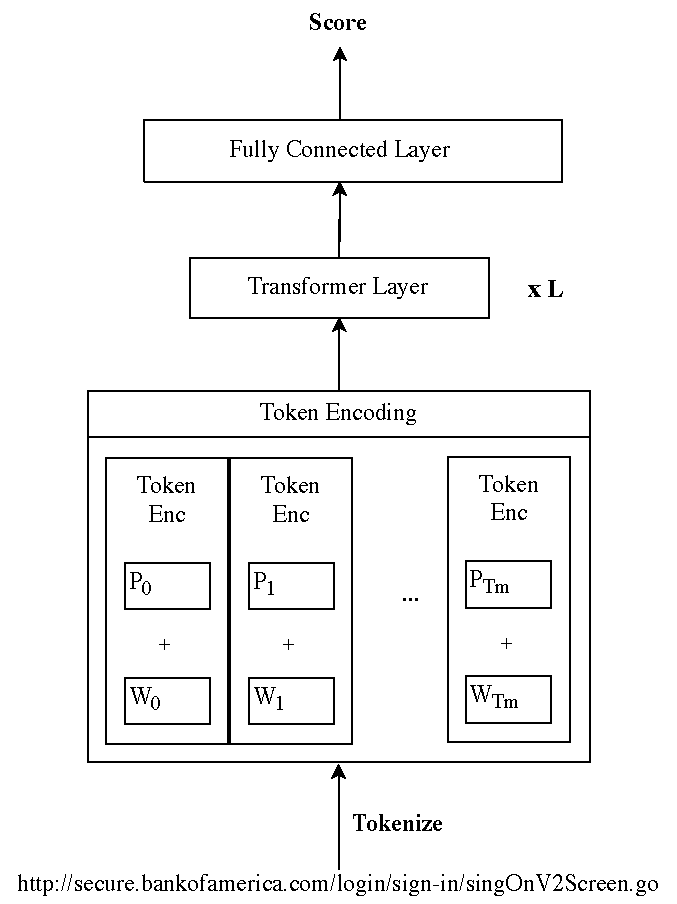
\includegraphics[width=0.4\linewidth]{urltran/figures/TransformerModel}
	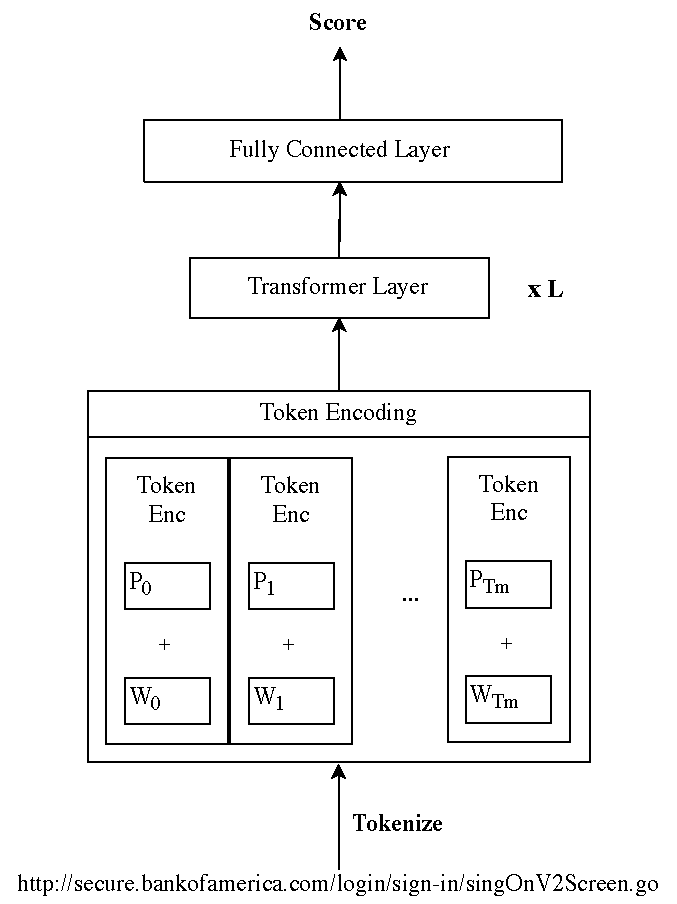
\includegraphics[width=0.4\linewidth,alt={Block diagram showing the inputs, tokenization, layers, and output of model.}]{urltran/figures/TransformerModel}
	\caption{\URLTranSys phishing URL detection model.}
	\label{fig:urltran:transformer}
\end{figure}
%\tagmcend\tagstructend
In the following sections, we first provide briefly summarize the transformer model architecture, followed by the training tasks used to train the model, and end with a description of the adversarial settings under which the best \URLTranSys model is evaluated and then trained with adversarial examples to improve its robustness.

\subsection{Architecture}
We describe the tokenization schemes and overall architecture for classification in this section, skipping a detailed description of transformer models for brevity.
Interested readers can review the transformer~\citep{vaswani2017attention}, BERT~\cite{devlin2019bert}, or RoBERTa~\citep{liu2019roberta} papers for details of the internal structure of transformer layers.

\subsubsection{Tokenization}
\label{sec:urltran:architecture:tokenization}
%
The raw input to the \URLTranSys model is the URL, which can be viewed as a text sequence.
The first step in the phishing URL detection task involves converting this input URL into a numerical vector which can be further processed by a classic machine learning or deep learning model.
Previous URL detection models~\citep{blum2020lexical} extracted lexical features by first splitting the URL with a set of important delimiters (e.g., `=', `/', `?', `.', ` ') and then creating a sparse binary features based on these tokens.
Recent deep learning-based URL detection models~\citep{le2018malicious,tajaddodianfar2020texception} instead include separate word-level and character-level CNNs where the character-level CNNs span different lengths of character subsequences.

Instead of these approaches, we experiment with multiple subword tokenization schemes in \URLTranSys.
Subword models have seen increased adoption in different tasks in NLP, including machine translation~\citep{sennrich2016neural}, word analogy~\citep{bojanowski2017enriching}, and question answering~\citep{zhang2019effective}.
Using subword models helps balance between the tradeoffs of using full-length words for each token (leading to fewer tokens required per input but a large token vocabulary) and character-based models (more tokens required per input but a smaller token vocabulary).
%allowing more input to be processed by a fixed-length model, 
%Using a subword model can provide morphological insights to improve inference.
For example, a full-length model would consider `bankofamerica' and `bankofcanada' as completely unrelated tokens, whereas a subword model can recognize the shared subword `bank' to correlate URLs belonging to the two banks.
Frequently occurring character substrings tend to correspond to subwords; common prefixes and suffixes can also provide relevant information.
%while being more robust to polymorphic attacks.
In particular, for fine-tuned \URLTranSysb and \URLTranSysr, we use the corresponding existing word piece~\citep{wu2016googles,devlin2019bert}  and Byte Pair Encoding (BPE) models~\citep{ratdford2019gpt2,liu2019roberta}, respectively.
In addition to these, we create custom character-level and byte-level BPE vocabularies using the training URL data to have a domain specific vocabulary for \URLTranSysc.
We test two different vocabulary sizes, 1K and 10K.
We tested  both sentence piece and BPE tokenization schemes in our models.
%as they attempt to find a balance of using both character substrings and full words and can capture unexpected unicode characters using their byte-level decomposition.


The BPE models first break the $m^{th}$ URL, $u_m$, into a sequence of text tokens, $\mathbf{TOK}_m$, where the individual tokens  may represent entire words or subwords~\citep{schuster2012japanese,sennrich2016neural,wu2016googles}.
Following the notation in~\cite{devlin2019bert}, the token sequence is formed as:
\begin{equation}
	\begin{split}
		& \mathbf{TOK}_m = \text{Tokenizer}(u_m)\\
	\end{split}
\label{eq:urltran:tok}
\end{equation}
%\end{comment}
\noindent where $\mathbf{TOK}_m$ is of length $T_m$ positions and consists of individual tokens ${Tok}_m^t$ at each position index $t$.
%${Tok}_t$ is an individual token generated from the $m^{th}$ URL generated by the wordpiece model.
For example, the BERT wordpiece token sequence generated from the URL of a popular banking login page,\\
\mbox{\small{$u_m$ = secure.bankofamerica.com/login/sign-in/signOnV2Screen.go}} \\
 is shown in Table~\ref{tab:urltran:boa}. The wordpiece model includes special text tokens specified by (\#\#) which build
 upon the previous token in the sequence. In the example in Table~\ref{tab:urltran:boa}, `\#\#of' refers to the continuation from s
 token (`bank'), and helps distinguish from the more common  separate token `of'.

\begin{table}
\centering
\resizebox{\linewidth}{!}{
\begin{tabular}{ll}
\hline
URL ($u_m$) & secure.bankofamerica.com/login/sign-in/signOnV2Screen.go \\
\hline
Token Sequence ($\mathbf{{TOK}_m}$) & \{ `secure', `.', `bank', `\#\#of', `\#\#ame', `\#\#rica', `.', `com', `/', `log', `\#\#in', `/', \\  & `sign', `-', `in', `/', `sign', `\#\#on', `\#\#v', `\#\#2', `\#\#screen', `.', `go' \} \\
  \hline
\end{tabular}
}
\caption{Example of the wordpiece token sequence extraction from a popular banking web page.}
\label{tab:urltran:boa}
\end{table}

\subsubsection{Classifier}
%
The final encoding produced by the transformer model can be used for a variety of downstream NLP tasks such
as language understanding, language inference, and question answering, and text classification.
We use the transformer embeddings for two tasks: pre-training masked language models, and fine-tuning for classification of phishing URLs.
Both of these tasks require a final representation layer which can be applied to multiple tokens for masked token prediction, and a pooled representation for classification.
The transformer models that we train use a single, dense two-class classification layer, which is applied to a special pooled token (`\texttt{[CLS]}') for classification. A dense layer having an output size equal to the size of the vocabulary of the tokenizer (\texttt{vocab\_size}) classes is used for predicting the masked token for the masked language modeling task during pre-training:

\begin{align}
	s_m = \sigma(\rmW_{p} \rvx_m^0 + \rvb_p) \label{eq:urltran:denseout}\\
	\rvs_m^t = \bm{\sigma} (\rmW_{v} \rvx_m^t + \rvb_v) \label{eq:urltran:denseword}
    %\label{eq:dense}
\end{align}

\noindent  In~(\ref{eq:urltran:denseout}), $\rmW_{p}$ and $\rvb$ are the weight matrix, bias vector respectively, for the final
dense linear layer for predicting the phising label.
$\sigma$ is the softmax function and 
 $s_m$ is the
score which predicts if the URL $\mathbf{u}_m$ corresponds to a phishing web page when performing classification.
Similarly, in~(\ref{eq:urltran:denseword}),
$\rvs_m^t, t \in [n]$ are 
 the sequence of masked token probability score vectors when performing masked language modeling for input token $\rvx_m^t$ computed using the softmax function $\bm{\sigma}$, with weight matrix $\rmW_{v}$ and bias vector $\rvb_v$.
 We now describe how input tokens are modified for masked language modeling and fine tuning.

\subsection{Training}
%
\subsubsection{Masked Language Modeling (MLM)}
The MLM task is commonly used to perform pre-training for transformers~\cite{devlin2019bert,liu2019roberta}. In this task, a random subset of tokens is replaced by a special `\texttt{[MASK]}' token.
 The training objective for the task is the cross-entropy loss corresponding to predicting the correct tokens at masked positions.
 The intuition for using this task for URLs is that specific query parameters and paths are generally associated with non-phishing URLs and therefore predicting masked tokens would help to uncover these associations.
 Similar intuitions derived from the cloze task~\cite{taylor1953cloze} motivate the usage of MLMs for pre-training natural language models.
Following the MLM hyperparameter settings for BERT, we selected 15\% of the tokens sampled uniformly for masking, of which 80\% are replaced, 10\% were left unchanged, and 10\% were replaced by a random vocabulary token at each iteration.
We used dynamic masking~\cite{liu2019roberta}, i.e., different tokens masked from the same sequence across iterations.
 Only the training subset of the full dataset was used for pre-training to prevent any data leakage. 

 \subsubsection{Fine Tuning}
 For \URLTranSysb and \URLTranSysr, we initialized all the parameters using the pretrained weights provided for BERT by \citet{devlin2019bert} and RoBERTa by \citet{liu2019roberta} respectively.
 For \URLTranSysc, we first pretrain each model using the MLM pretraining task and use the learned weights as initialization values.
 Next, each \URLTranSys model, is trained
 using a second ``fine-tuning'' task using the error backpropagated from the URL classification task.
 We used the Adam~\cite{kingma2014adam} optimizer with cross-entropy losses to train each model.
 
 \subsection{Adversarial Attacks and Data Augmentation}
 \label{sec:urltran:adv_attack}
%\pmcomment{Potentially discuss covariate shift here?}
 
\textbf{Threat Model}
%\pmcomment{Consider rewording this seciton}
The approach we use for generating data for an adversarial attack includes generating separate augmented training, validation and test datasets based on their original dataset.%~\cite{Goodfellow2014}.
For each URL processed in these datasets, we generate
a random number. If it is less than 0.5, we augment the URL, or otherwise, we include it in its original form. For URLs which are to be augmented,
we modify it using either a homoglyph attack, a compound attack or parameter reordering with equal probability. If a URL has been augmented,
we also include the original URL in the augmented dataset. 

The threat model for \URLTranSys allows for the attacker to create any phishing URL including those which employ domain squatting techniques. In its current form, \URLTranSys is protected against homoglyph and compound word attacks through dataset augmentation.
However, any domain squatting attacks can also be simulated and included in the augmented adversarial training, validation, and test sets. 
In addition, a larger number of adversarial training examples can be directed at more popular domains such as https://www.bankofamerica.com that may be a target of attackers.
We assume that inference can be executed by the countermeasure system prior to the user visiting the unknown page. 
This can be done by the email system at scale by evaluating multiple URLs in parallel. In our evaluation, we found that \URLTranSys requires 0.36096 milliseconds per URL on average which is a reasonable amount of latency.
 
 \textbf{Adversarial Testing}
 Data augmentation using invariants, contextual replacement, and reward-based learning has been used to improve classifiers in the text domain~\citep{kobayashi2018contextual,hu2019learning}.
 These can be extended to augment data in the URL domain.
 Phishing URL attacks can occur on short-lived domains and URLs which have small differences from existing, legitimate domains.
 We simulate two attack scenarios by constructing examples of such adversaries based on modifying benign URLs.
 Note that these generated domains do not actually exist in the pre-existing training and testing data, but are based upon frequently observed phishing attack patterns.
 We also utilized a reordering-based augmentation, which is used is used to generate benign perturbations for evaluating robustness of adversarially trained models.

 \subsubsection{Homoglyph Attack}
We generated domains that appear nearly identical to legitimate URLs by substituting characters with other unicode characters that are similar in appearance.
This attack strategy is commonly referred to as a \textit{homoglyph attack}~\cite{ji2018deepwordbug,yerima2020high}, and
we implement this strategy using the \texttt{homoglyphs}\footnote{https://pypi.org/project/homoglyphs/} python library.
In particular, given a URL, we first extract the domain.
For a randomly selected character in the domain, we check for one unicode (utf-8) Latin or Cyrillic character that is a homoglyph for it. 
For each perturbed URL, we selected a random character to perturb and generated the associated URL, labeled as a phishing URL.
We replaced the character by its homoglyph to construct a new URL.
%We only perturb one character to minimize the probability that such a URL would we be identified as phishing by the user.
%The URLs generated from this strategy are labeled as phishing.

\subsubsection{Compound Attack}
An alternative way to construct new phishing URLs is by splitting domains into sub-words (restricted to English) and then concatenating the sub-words with an intermediate hyphen.
For example, `bankofamerica.com' $\rightarrow$ `bank-of-america.com'.
To implement this, we leveraged a popular dictionary used by multiple spell check programs, the \texttt{enchant} dictionary\footnote{https://pypi.org/project/pyenchant/}.
Consider a URL with domain $d$ having $|d| = n$ characters.
Let $\gD$ denote the \texttt{enchant} English dictionary.
Let $C(d, i, j)$ denote the function that returns True if $d[i \dots j]$ can be split into one or more parts, each of which is a word in the dictionary $\gD$.
The compound word problem can be formulated recursively as
\begin{align}
	C(d, i, j) =
	\begin{cases}
		\text{True}, & d[i \dots j] \in \gD\\
		\text{True} & \exists k, C(d, i, k) \text{ and } C(d, k+1, j)\\
		\text{False} & \text{otherwise}
	\end{cases}
\end{align}
Using this recursive definition, we implemented a dynamic programming algorithm that can compute whether a domain can be split and the corresponding splits.
%\pmcomment{Maybe add the dynamic program algorithm here, and talk about the computational complexity?}
These splits are then concatenated with hyphens between the discovered words.
Note that the base case check  $d[i\dots j] \in \gD$ is performed in a case insensitive manner to ensure that the dictionary checks do not miss proper nouns.

\newcommand{\permuteSys}{PermuteURL\xspace}
\subsubsection{Parameter Reordering}
Forms of permutation=based denoising have shown improvements for langauge modeling~\cite{lewis2020bart} and machine translation~\cite{lample2018unsupervised}.
We adapt these intuitions into the phishing URL domain.
As the query parameters of a URL are interpreted as a key-value dictionary, this augmentation incorporates permutation invariance. 
An example of a URL and permutation is provided in Figure~\ref{fig:urltran:permute_url}.
We use this approach to generate benign examples.
Reordering the parameters still results in a valid URL, i.e., parameter reordering does not represent a phishing attack, and therefore we do not modify the label.
\begin{figure}
	\centering
	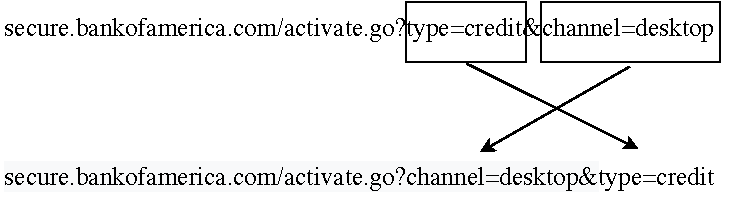
\includegraphics[width=0.75\linewidth,alt=Example of GET paramter reordering for a URL.]{urltran/figures/PermuteURL}
	\caption{An example of parameter reordering}
	\label{fig:urltran:permute_url}
\end{figure} 


 

\section{Evaluation}
\label{sec:urltran:eval}
%
We now present the numerical evaluation of the different approaches presented in the previous sections.
Thereafter, we compare \URLTranSys to several recently proposed baselines.
We also report the model's training and inference times.
Finally, we analyze the robustness of the model \textit{adversarial test}  URLs.


\noindent\textbf{Setup:}
In our experiments, we set the hyperparameters for previously published models according to their settings in the original paper.
For evaluating \URLTranSysc, we vary the number of layers between $\{3, 6, 12\}$, vary the number of tokens per input URL sequence between $\{128, 256\}$.
We use both a byte-level and character-level BPE tokenizer with 1K- and 10K-sized vocabularies.
We randomly pick 15 hyperparameter combinations among these settings and present the results for these.
The Adam optimizer~\citep{kingma2014adam} is used in both pre-training and fine-tuning, with the triangular scheduler~\citep{smith2017cyclical} used for fine-tuning.
The hyperparameter settings for all models are provided in Section~\ref{sec:urltran:hyper}.
All training and inference experiments were conducted using PyTorch~\citep{pytorch} version 1.2 with NVIDIA Cuda 10.0 and Python 3.6.
The experiments were performed by extending the HuggingFace and Fairseq PyTorch implementations found on GitHub~\citep{huggingface,fairseq}.
Given the large class imbalance, accuracy is a poor metric of model performance.
To supplement accuracy, we evaluated all the models using the true positive rate (TPR) at low false positive rate (FPR) thresholds. 
We used the receiver operating characteristics (ROC) curve to compute this metric.


\noindent\textbf{Baselines:}
To evaluate the performance of our models, we compared them to two baseline phishing URL detection models: URLNet and Texception. URLNet~\citep{le2018malicious} is a CNN-based model which was recently proposed for the task of detecting URLs which identify malicious web sites. 
For comparison purposes, we trained and tested the URLNet model for the detection of phishing URLs.
Texception~\citep{tajaddodianfar2020texception} is another deep learning URL detection model for the task of identifying phishing URLs. 
Note that \citet{tajaddodianfar2020texception} compared Texception to a Logistic Regression-based model and found that Texception offered better performance.
Thus, we did not repeat that baseline experiment in this work.

\subsection{End-to-end Training}
%\noindent\textbf{\URLTranSysc.}
Transformers typically require large amounts of pre-training data (e.g., BERT~\citep{devlin2019bert} used a corpus of  $\approx$ 3.3 B tokens).
However, this data is derived from text articles, which are structured differently from URLs.
We trained the \URLTranSysc model based solely on the URL data found in our datasets to compare the results of finetuning using BERT (\URLTranSysb) and RoBERTa (\URLTranSysc) pretrained models to models pretrained only on in-domain URL data. 
The difference in dataset size and data domain make it important to understand the impact of different hyperparameters used when training transformers from scratch.
We compared runs across different hyperparameters on the basis of area under ROC (AUROC) and TPR@0.01\% FPR.
Figure~\ref{fig:urltran:pretrain_scratch} demonstrates that the training is not very sensitive to sequence length. 
Smaller byte-level vocabularies tend to be better overall, but at low FPR, the difference is not significant.
Finally, we found that the 3 layer model generalized the best.
We hypothesize that the better performance of the model with fewer layers is because of limited pre-training data.%\todo{pre-training vs pretraining consistent}
In the next few sections, we validate this hypothesis by evaluating fine-tuned model (\URLTranSysb, \URLTranSysr) that are tuned on a larger dataset.

\begin{figure}
\begin{subfigure}{0.8\linewidth}
	\centering
    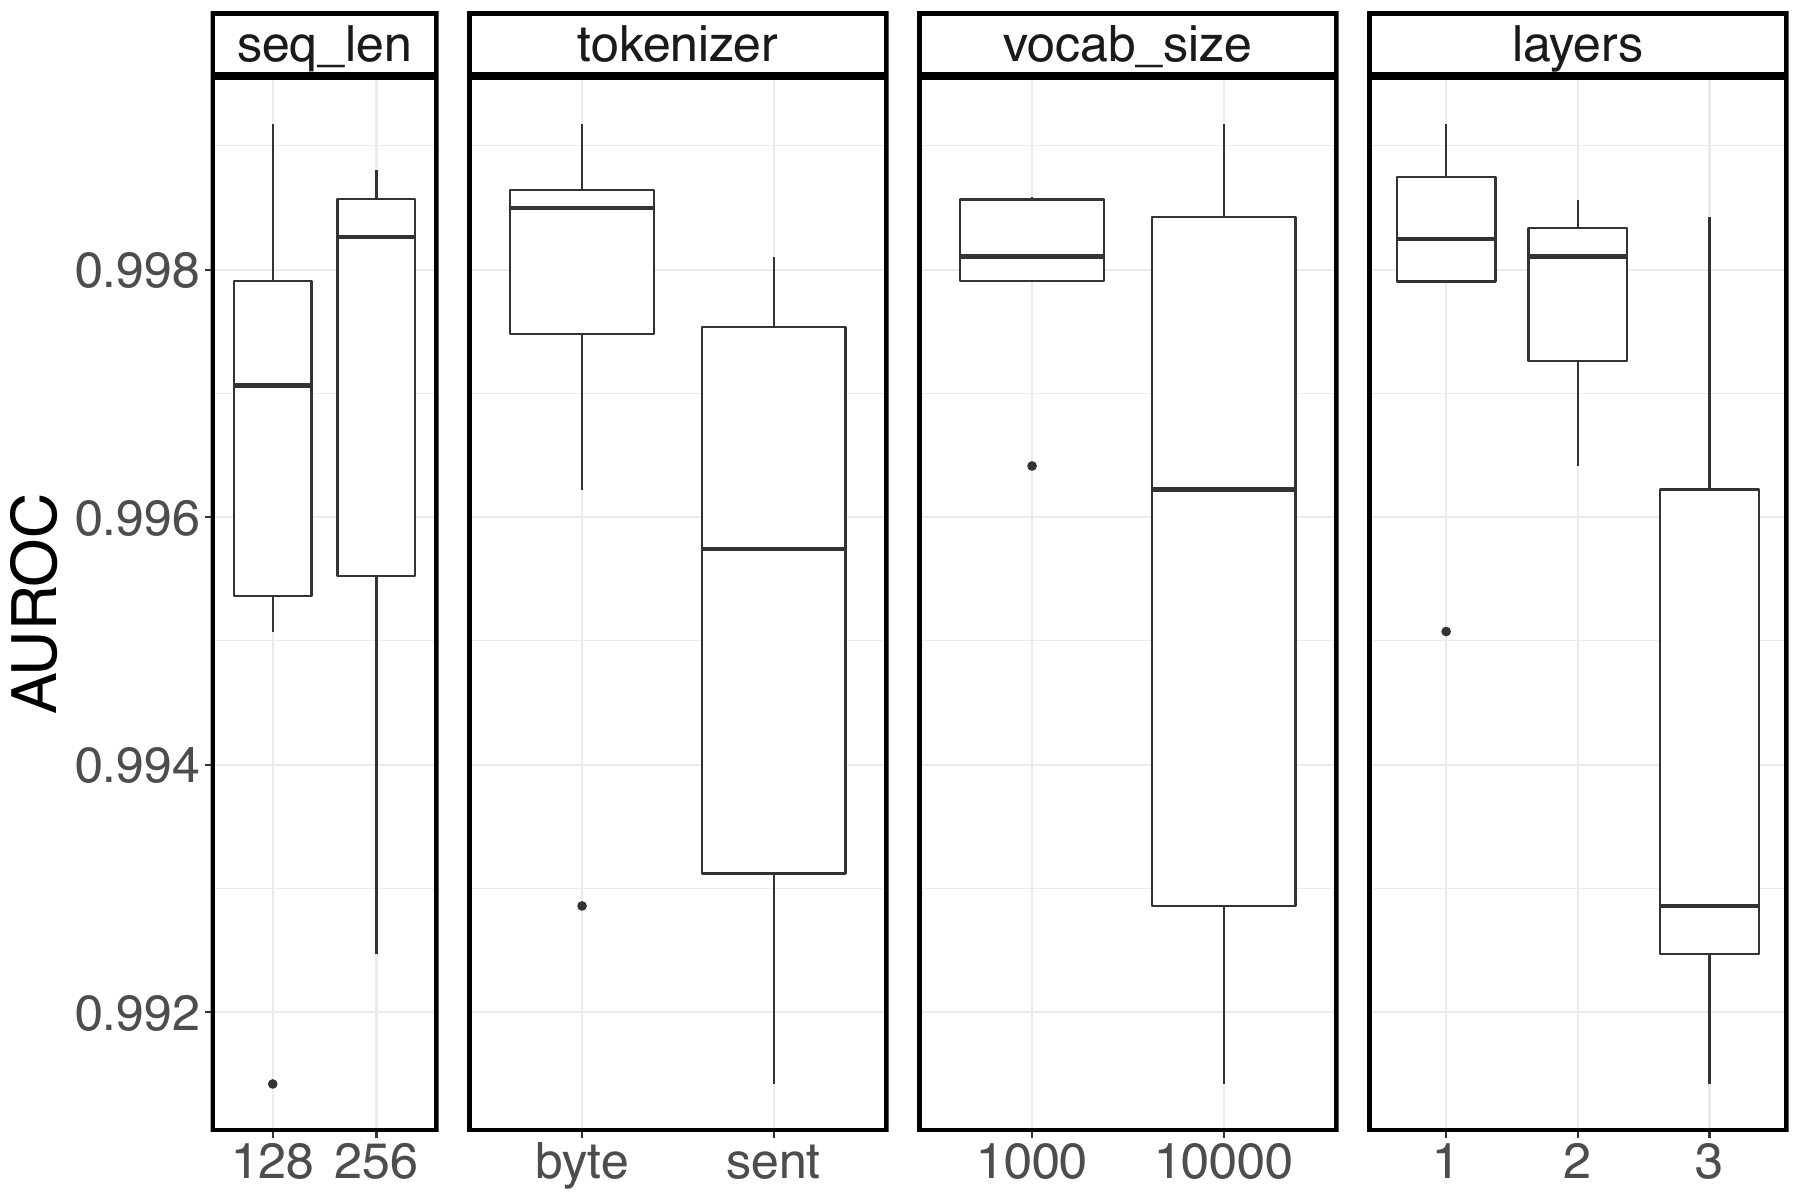
\includegraphics[width=0.95\linewidth,alt={Box plots for area under ROC comparison for different seq len, tokenizers, vocab size, and layers.}]{urltran/figures/roc_hyperparams.png}
\caption{Area under ROC vs hyperparameters}
\label{fig:urltran:pretrain_scratch:roc}
\end{subfigure}
\begin{subfigure}{0.8\linewidth}
	\centering
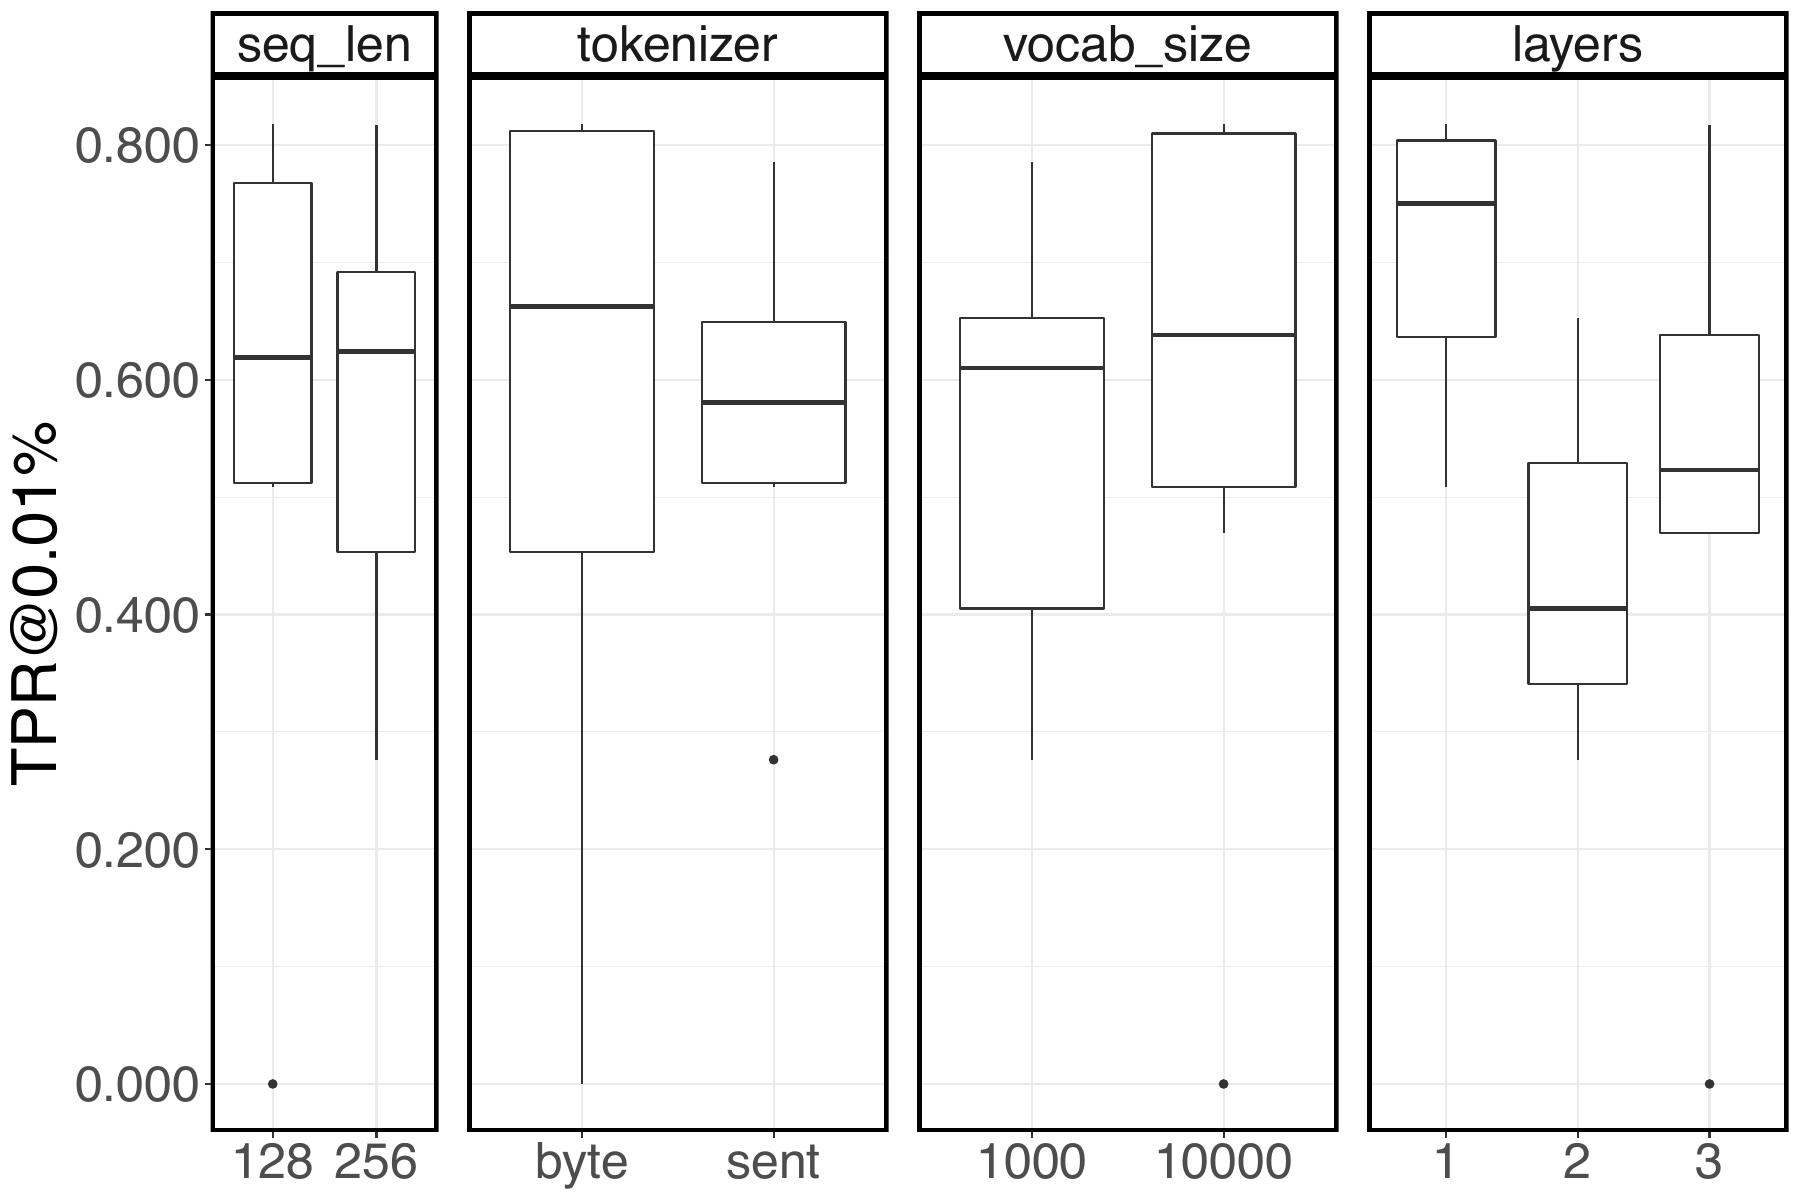
\includegraphics[width=0.95\linewidth,alt={Box plots for TPR@FPR=0.01\% comparison across different seq len, tokenizers, vocab size, and layers.}]{urltran/figures/tpr_0.01_hyperparams.png}
\caption{TPR@FPR = 0.01\% vs hyperparmeters}
\label{fig:urltran:pretrain_scratch:tpr}
\end{subfigure}
\caption{Variance in quality of \URLTranSysc across different hyperparameter settings}\
\label{fig:urltran:pretrain_scratch}
\end{figure}


\subsection{Numerical Evaluation}


\begin{figure}
    \centering
	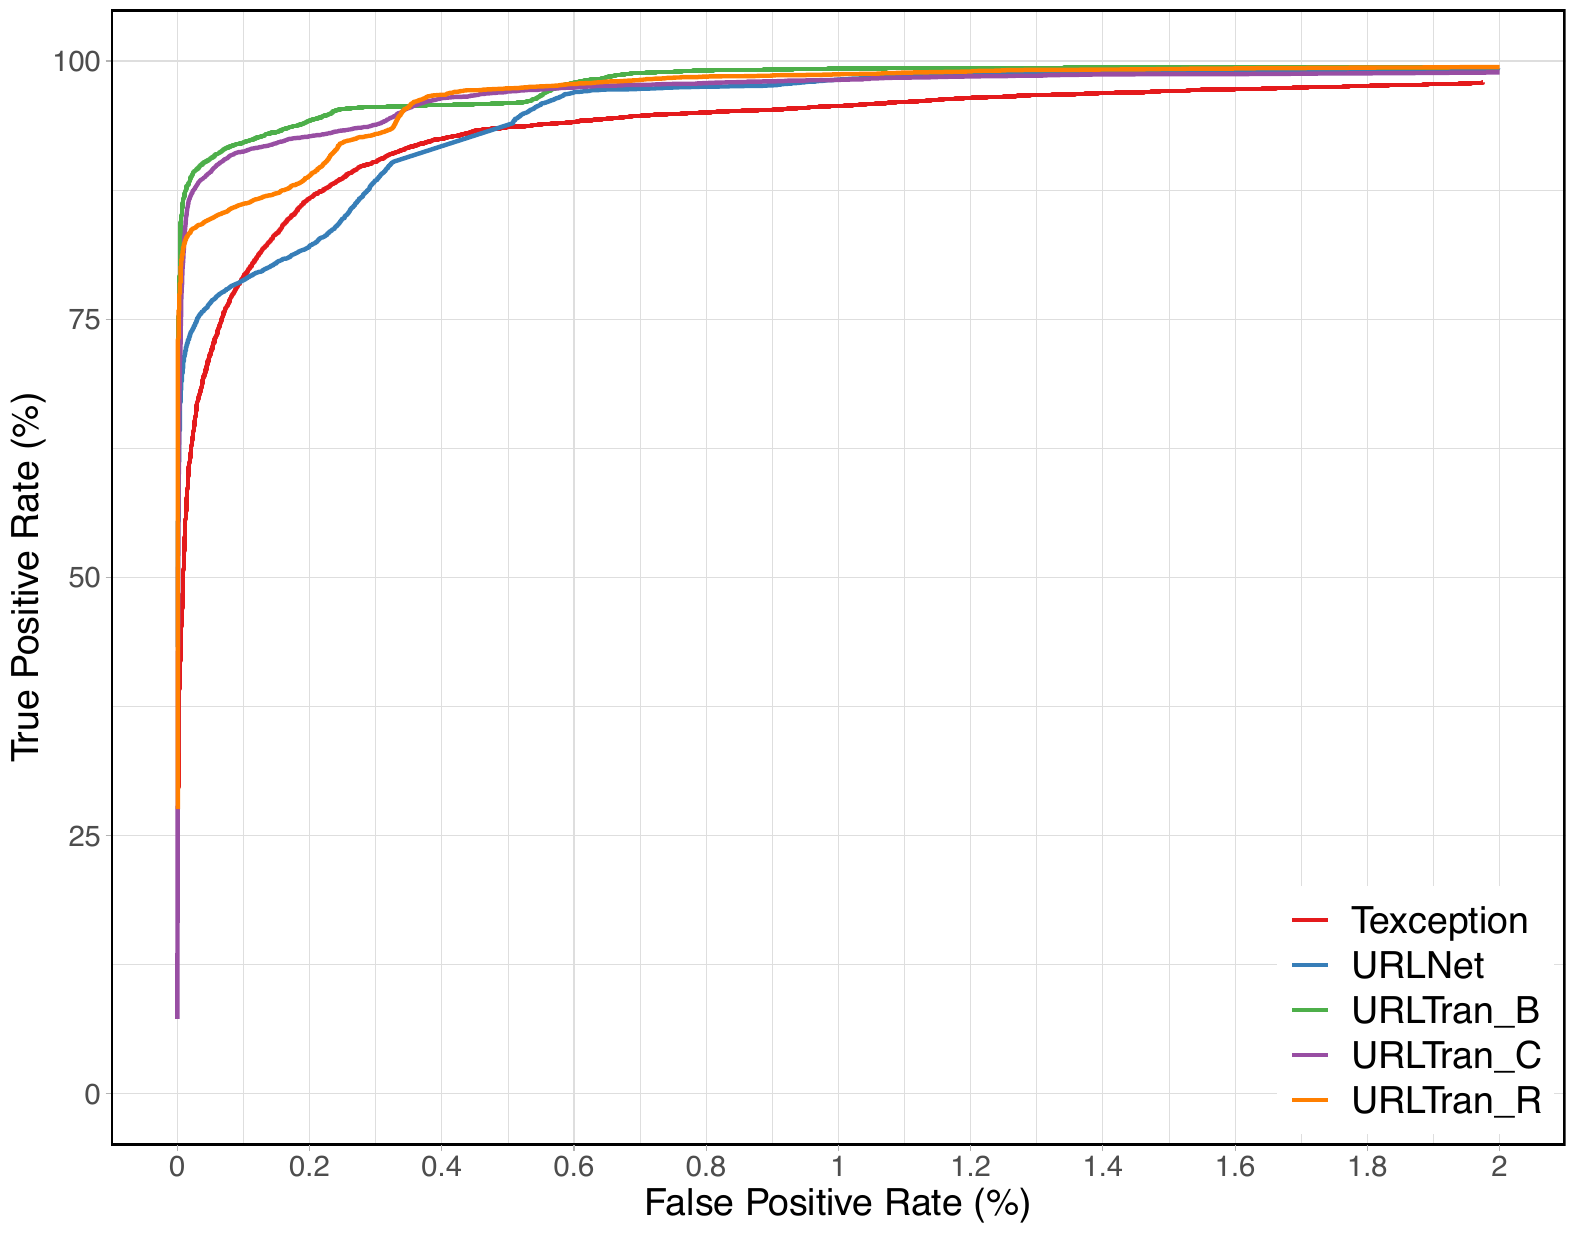
\includegraphics[width=0.7\linewidth,alt={ROC curev indicating impromvents of our model over baseline models upto a maximum of 2\% FPR}]{urltran/figures/roc_0_02_R.png}
	\caption{Receiver operating characteristic curve indicating the performance of the \URLTranSys and several baseline models zoomed into a maximum of 2\% false positive rate.}
	\label{fig:urltran:transformer2}
\end{figure}

\begin{figure}
    \centering
	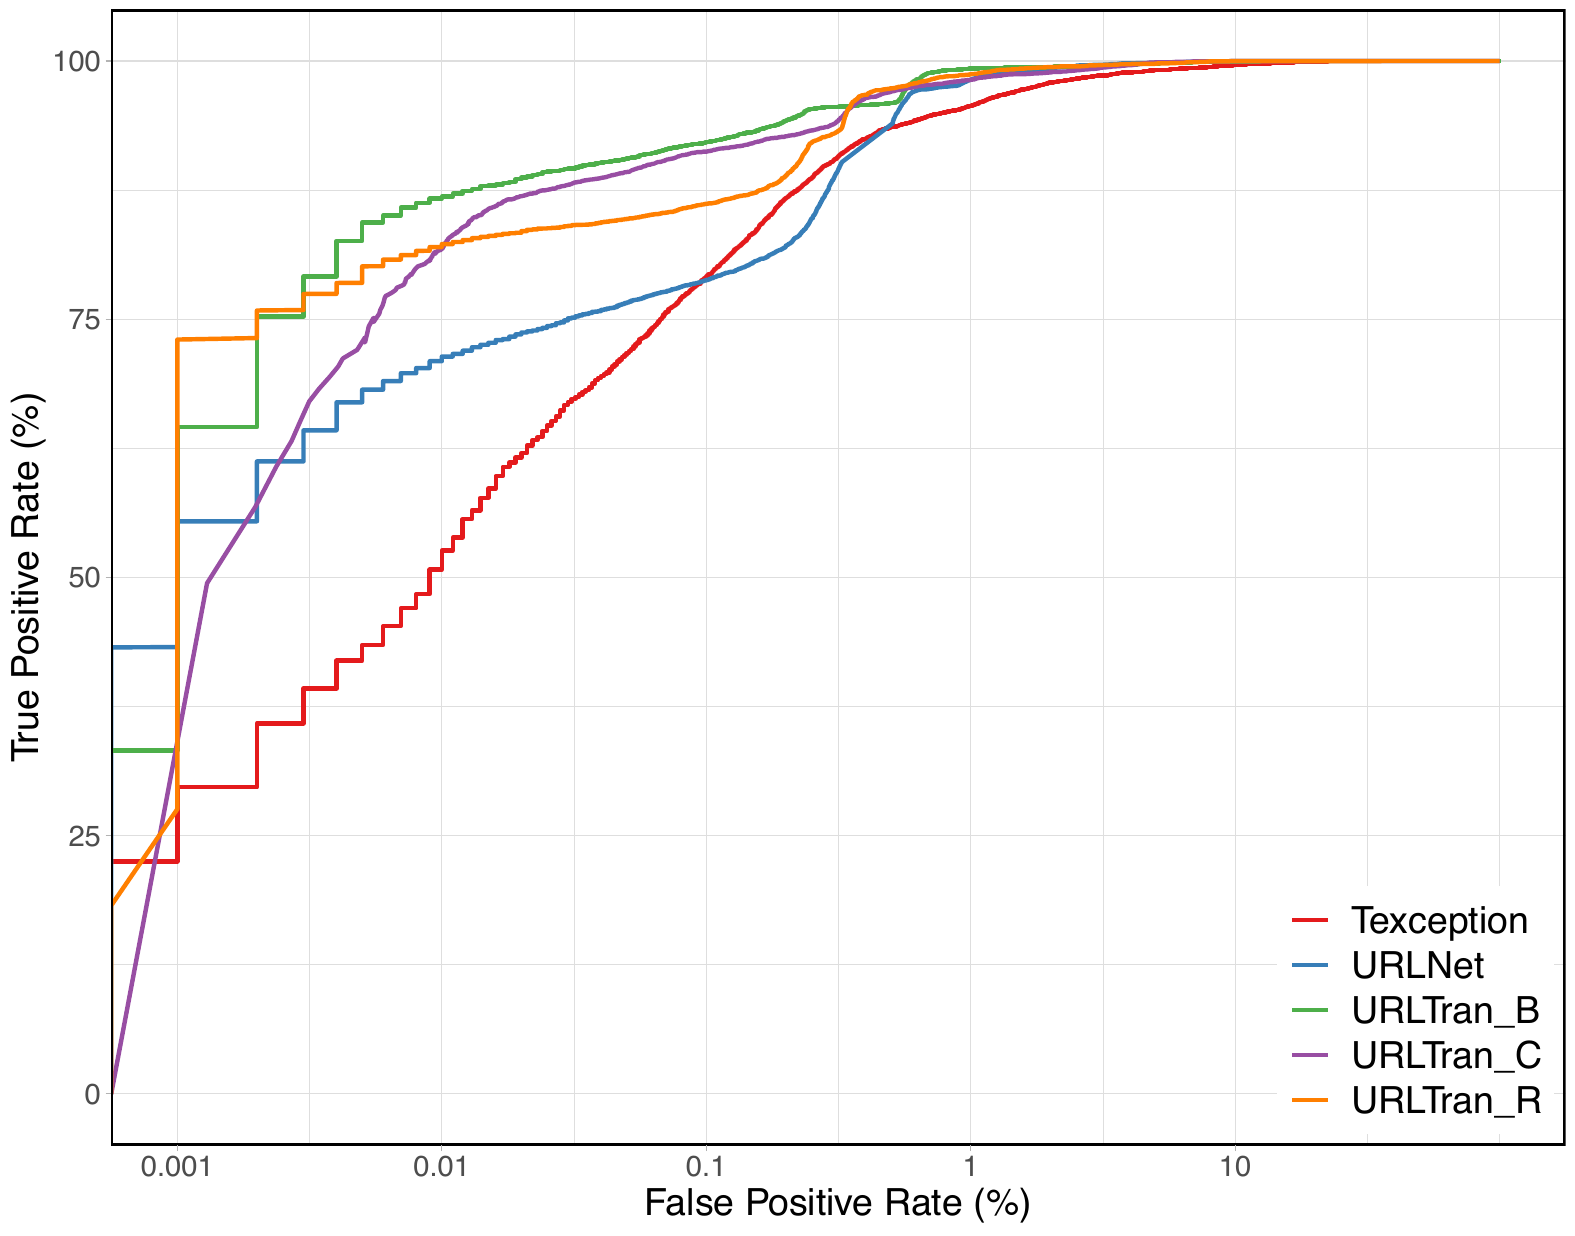
\includegraphics[width=0.7\linewidth,alt={Zoomed in full ROC curve with a log x-axis.}]{urltran/figures/log_roc_R.png}
	\caption{Zoomed in receiver operating characteristic curve with a log x-axis.}
	\label{fig:urltran:log_transformer2}
\end{figure}



\noindent\textbf{Model Performance.}
We next analyzed the performance of the best parameters of all the proposed transformer variants.
To understand how these models compare at \textit{very low FPRs} where detection thresholds must be set to operate in a production environment, we first plotted the ROC curves on a linear x-axis zoomed into a 2\% maximum FPR in Figure~\ref{fig:urltran:transformer2}.
We also re-plot these ROC curves on a log x-axis in the semilog plot in Figure~\ref{fig:urltran:log_transformer2}.
These results indicate that all variants of \URLTranSys offer a significantly better
true positive rate over a wide range of extremely low FPRs. In particular, \URLTranSys matches or exceeds the TPR of URLNet for the FPR range of 0.001\% - 0.75\%.
The result is very important because phishing URL detection models must operate at very low FPRs (e.g., 0.01\%) in order to minimize the number of times the security service predicts that a benign URL is a phishing site (i.e., a false positive). In practice, the browser manufacturer selects the desired FPR and tries to develop new models which can increase the TPR for the selected FPR value.
Note that TPR@FPR is the standard metric commonly used both in production settings and in prior art such as Texception and URLNet.
In addition to the ROC curve analysis, we also summarize a number of key performance metrics in Table~\ref{tab:urltran:model-perf}, where `F1' is the F1 score, and `AUC' is the area under the model's ROC curve.
The proposed \URLTranSys model outperforms both Texception and URLNet for all of these metrics.
In particular, we note that  at an FPR
of 0.01\%, \URLTranSysb has a
TPR of 86.80\% compared to 71.20\% for URLNet and 52.15\% for Texception.

\begin{table}[ht]
\begin{center}
\resizebox{\linewidth}{!}{
\begin{tabular}{ccccccc}
\toprule
Model & Accuracy (\%) & Precision (\%) & Recall (\%) & TPR@FPR=0.01\% & F1 & AUC \\
\midrule
Texception & 99.6594 & 99.7562 & 99.6594 & 52.1505 & 0.9969 & 0.9977 \\
URLNet & 99.4512 & 99.7157 & 99.4512 & 71.1965 & 0.9954 & 0.9988 \\
\URLTranSysc & 99.5983 & 99.7615 & 99.5983 & 81.8577 & 0.9965 & 0.9992 \\
\URLTranSysr & 99.6384 & 99.7688 & 99.6384 & 82.0636 & 0.9968 & 0.9992 \\
\URLTranSysb & 99.6721 & 99.7845 & 99.6721 & 86.7994 & 0.9971 & 0.9993 \\
\bottomrule
\end{tabular}
}
\end{center}
\caption {Comparison of different performance metrics for \URLTranSys and the two baseline models.}
\label{tab:urltran:model-perf}
\end{table}


%\input{error}

\noindent\textbf{Training and Inference Times.}
The total time required to train the best \URLTranSysb model was 4:57:11 on an NVIDIA V100. Inference
required 0:10::44 to complete for an average of 0.36096 milliseconds per sample.


\begin{figure}
    \centering
	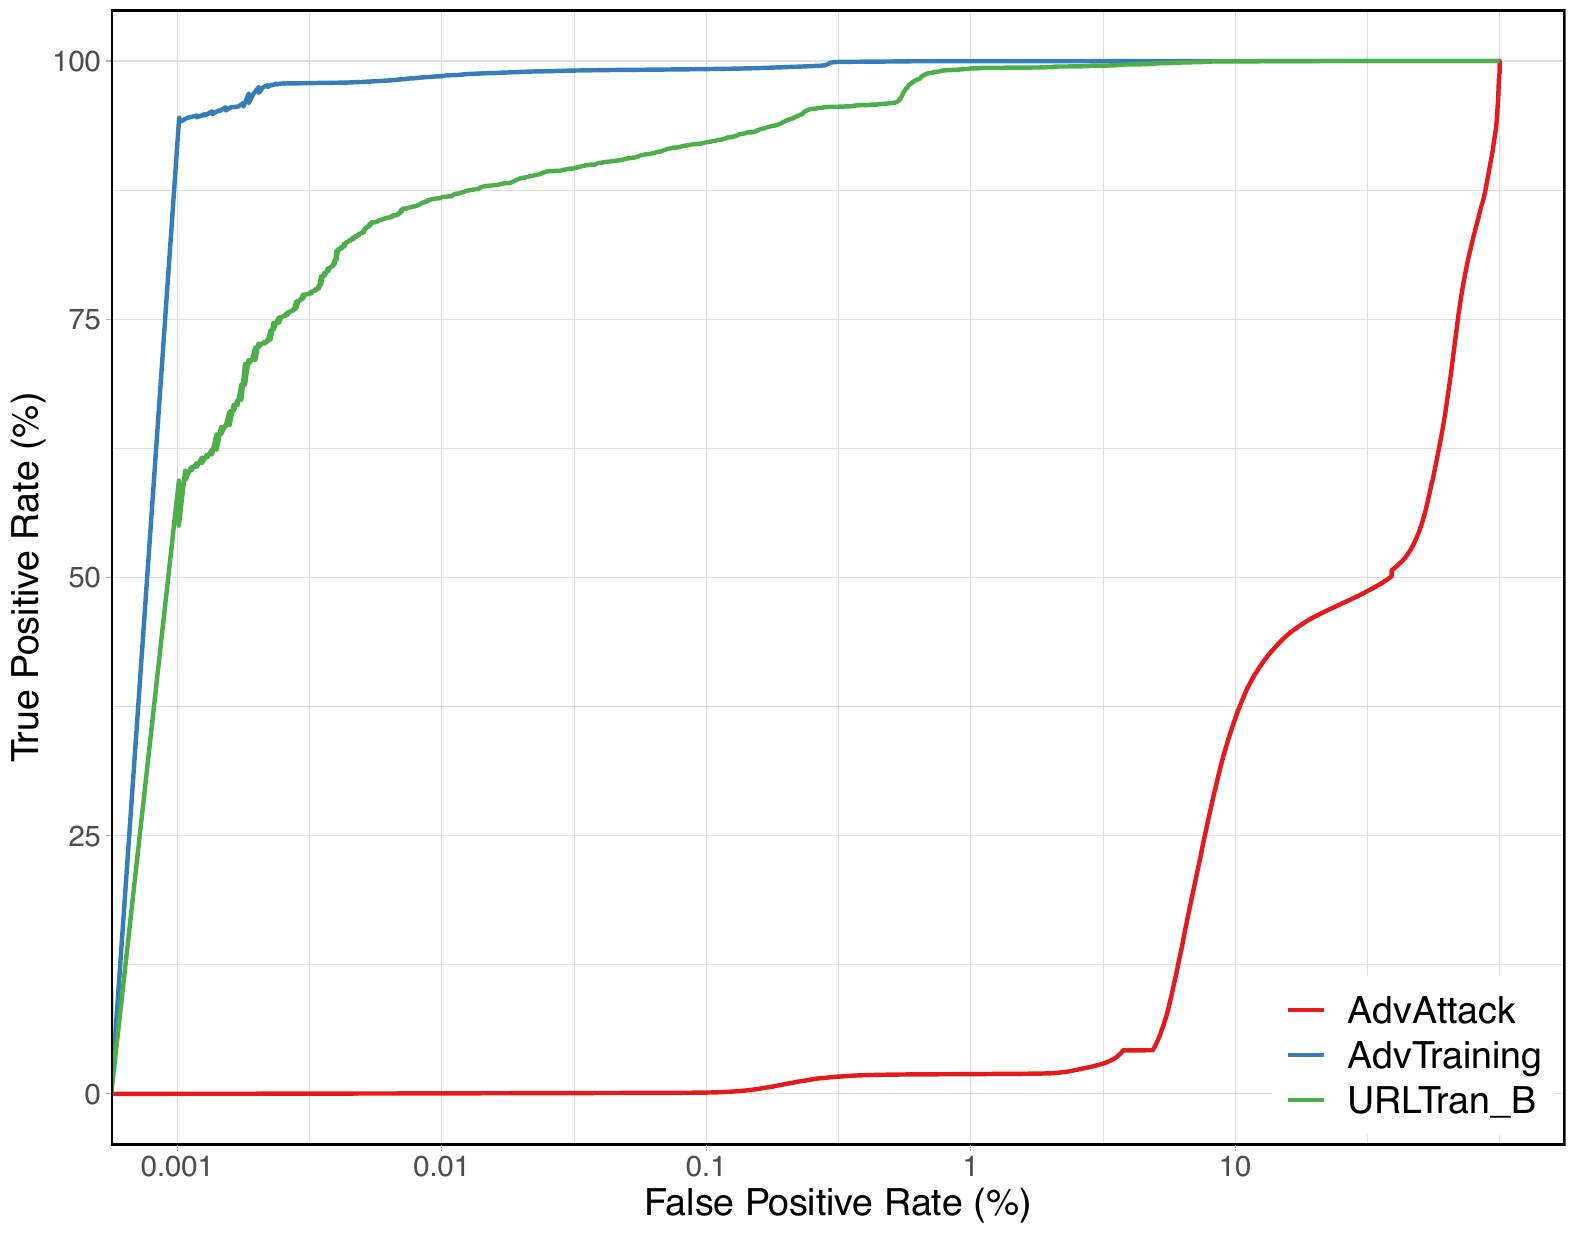
\includegraphics[width=0.7\linewidth,alt={ROC curve under adversarial attack and robustness after training with augmented data.}]{urltran/figures/log_roc_adv_R.png}
	\caption{ROC curve for \URLTranSysb when under adversarial attack, and adversarial robustness after augmented training}
	\label{fig:urltran:adversarial_roc}
\end{figure} 

\subsection{Adversarial Evaluation.}
To understand \URLTranSys's robustness to adversarial attacks, we first compared the low FPR regions of the ROC curve of the unprotected model tested with the original test set to the
test set which includes adversarial samples (AdvAttack) generated through the methods described in Section~\ref{sec:urltran:adv_attack} (Figure~\ref{fig:urltran:adversarial_roc}).
There is a significant drop in performance of \URLTranSysb when attacked with adversarial URLs.
As discussed previously (Section~\ref{sec:urltran:adv_attack}, \textit{adversarial testing} provides a mechanism to ensure that models can be made robust to attacks that follow known threat models.
We test this hypothesis by considering the scenario where attack strategies are incorporated into the training data (AdvTraining).
%\pmcomment{Another place where covariate shift can be referenced.}
On the addition of adversarial attack patterns to the training, the model is able to  the adapt to novel attacks, and even exceeded the performance of the non-adversarially trained version of \URLTranSys.
These results demonstrate that  creating adversarial can help models such as \URLTranSys adapt to unseen attacks.
Further, as new attack strategies are recognized (e.g., alternative homoglyph), a robust version of \URLTranSys can be trained to recognize similar patterns in unseen test data.

\section{Hyperparameter Settings}
\label{sec:urltran:hyper}
For replicability, this sectino provides the hyperparameter settings for the three variants of the proposed \URLTranSys model as well as those for two baseline models.
Tables~\ref{tab:urltran:URLNetParams} and~\ref{tab:urltran:TexParams} list the hyperparameters for the URLNet and Texception models that we use
as baselines in our study. The hyperparameter settings for the best performing \URLTranSysb model are provided in Table~\ref{tab:urltran:TransParamsBert}.
In addition, the best hyperparameter settings for the \URLTranSysr and \URLTranSysc are given in Tables~\ref{tab:urltran:TransParamsRoberta} and~\ref{tab:urltran:TransParamsCustVoc},
respectively.

\begin{table}
\centering
\footnotesize
\begin{tabular}{lc}
\toprule
Parameter & Value \\
\midrule
max\_len\_words & 200 \\
max\_len\_chars & 1000 \\
max\_len\_subwords & 20 \\
min\_word\_freq & 1 \\
dev\_pct & 0.001 \\
delimit\_mode & 1 \\
emb\_dim & 32 \\
filter\_sizes & {[}3,4,5,6{]} \\
default\_emb\_mode & char + wordCNN \\
nb\_epochs & 5 \\
train\_batch\_size & 128 \\
train\_l2\_reg\_lambda & 0.0 \\
train\_lr & 0.001 \\
\bottomrule
\end{tabular}
\caption{Hyperparameters used for URLNet.}
\label{tab:urltran:URLNetParams}
\end{table}


\begin{table}
\centering
\footnotesize
\begin{tabular}{clc}
\toprule
\multicolumn{2}{c}{Parameter} & Value\\
\midrule
\multirow{5}{*}{
\vtop{\hbox{\strut Characters}\hbox{\strut Branch}}
} & embedding dimension & 32 \\
 & number of blocks & 1\\
 & block filters & {[}2,3,4,5{]}\\
 & Adaptive MaxPool output & 32,32\\
 & maximum characters & 1000\\
\midrule
\multirow{5}{*}{
 \vtop{\hbox{\strut Words}\hbox{\strut Branch}}
} & embedding dimension & 32\\
 & number of blocks & 1\\
 & block filters & {[}1,3,5{]}\\
 & Adaptive MaxPool output & 32,16\\
 & maximum words & 50\\
\midrule
\multirow{6}{*}{
\vtop{\hbox{\strut FastText}\hbox{\strut Model}}
} & minimum words to include & 50\\
 & vocabulary size & 120000\\
 & window size & 7\\
 & n-grams & 2-6\\
 & embedding dimension & 32\\
 & epochs trained & 30\\
\bottomrule
\end{tabular}
\caption{Hyperparameters used for Texception.}
\label{tab:urltran:TexParams}
\end{table}

\begin{table}
\centering
\footnotesize
\begin{tabular}{lc}
\toprule
Parameter & Value \\
\midrule
  attention probs dropout prob & 0.1 \\
  hidden act & gelu \\
  hidden dropout prob & 0.1 \\
  hidden size & 768 \\
  initializer range & 0.02 \\
  intermediate size & 3072 \\
  layer norm eps & 1e-12 \\
  max position embeddings & 512 \\
  num attention heads & 12 \\
  num hidden layers & 12 \\
  type vocab size & 2 \\
  vocab size & 30522 \\
  bert model & bert-base-uncased \\
  max seq length & 128 \\
  train batch size & 32 \\
  learning rate & 2e-5 \\
  num train epochs & 10 \\
  \bottomrule
\end{tabular}
\caption{Hyperparameters  used for training the proposed Huggingface-based \URLTranSysb model.}
\label{tab:urltran:TransParamsBert}
\end{table}

\begin{table}
\centering
\footnotesize
\begin{tabular}{lc}
\toprule
Parameter & Value \\
\midrule
Number of Layers & 12 \\
Hidden size & 768 \\
FFN inner hidden size & 3072 \\
Attention heads & 12 \\
Attention head size & 64 \\
Dropout & 0.1 \\
Attention Dropout & 0.1 \\
Warmup Steps & 508 \\
Peak Learning Rate & 1e-4 \\
Batch Size & 2k \\
Max Epochs & 10 \\
Learning Rate Decay & Linear \\
Adam $\epsilon$ & 1e-6 \\
Adam $\beta_1$ & 0.9 \\
Adam $\beta_2$ & 0.98 \\
Gradient Clipping & 0.0 \\
Tokens per sample & 256 \\
\bottomrule
\end{tabular}
\caption{Hyperparameters used for fine-tuning the proposed Fairseq-based \URLTranSysr model.}
\label{tab:urltran:TransParamsRoberta}
\end{table}

\begin{table}
\begin{subtable}{0.45\linewidth}
    \footnotesize
    \centering
    \begin{tabular}{lc}
        \toprule
        Parameter & Value \\
        \midrule
        Number of Layers & 3 \\
        Hidden size & 768 \\
        FFN inner hidden size & 3072 \\
        Attention heads & 12 \\
        Attention head size & 64 \\
        Dropout & 0.1 \\
        Attention Dropout & 0.1 \\
        Tokens per sample & 128 \\
        Peak Learning Rate & 1e-4 \\
        Batch Size & 2k \\
        Tokenizer Type & Byte BPE\\
        Weight Decay & 0.01 \\
        Max Epochs & 30 \\
        \multirow{2}{*}{Learning Rate Decay} & reduce \\
         & on plateau \\
        LR Shrink & 0.5 \\
        Adam $\epsilon$ & 1e-6 \\
        Adam $\beta_1$ & 0.9 \\
        Adam $\beta_2$ & 0.98 \\
        Gradient Clipping & 0.0 \\
        Learning Rate & 1e-4 \\
        vocab size & 10000 \\
      \bottomrule
    \end{tabular}
\end{subtable} %
\begin{subtable}{0.45\linewidth}
    \footnotesize
    \centering
	\begin{tabular}{lc}
        \toprule
		Parameter & Value \\
        \midrule
		Learning Rate & 1e-4 \\
		Batch Size & 2k \\
		Max Epochs & 10 \\
		Learning  & \multirow{2}{*}{Linear} \\
		Rate Decay & \\
		Warmup ratio & 0.06 \\
		\bottomrule
	\end{tabular}
\end{subtable}
\caption{Hyperparameters used for pre-training (left) and fine-tuning (right) the proposed \URLTranSysc model.}
\label{tab:urltran:TransParamsCustVoc}
\end{table}

\section{Conclusion}
\label{sec:conc}
%
This work focused on the \textit{pre-deplyment} stage for building more adaptive models by incorporating \textit{adversarial testing}.
We have proposed a new transformer-based system called \URLTranSys whose goal is to predict the label of an unknown URL one which either references a phishing or a benign web page.
Transformers have demonstrated state-of-the-art performance in many natural language processing tasks, and the secnd objective of this work is to understand if these methods can also work well in the cybersecurity domain.
We demonstrated that transformers which are fine-tuned using standard BERT tasks and a BPE tokenizer also work remarkably well for the task of predicting phishing URLs.
%Instead of extracting lexical features or using CNNs kernels which span multiple characters and words, common in previously proposed URL detection models, our system used BPE tokenizers for this task. 
%Next, transformers convert the token sequence to an embedding vector which can then be used as input to a dense linear layer.
Results indicate that \URLTranSys was able to significantly outperform recent baselines, particularly over a wide range of very low false positive rates.
We also demonstrated that transformers can be made robust to novel attacks under specific threat models when we adversarially augment the training data used for training them. 

\endinput